%% main_report38.tex
%% SAMBP TR-38/2026: GFL vs GFM Inverter Fault Characterisation
%%
%% pdflatex main_report38.tex

\documentclass[11pt,a4paper]{article}

\usepackage[T1]{fontenc}
\usepackage[utf8]{inputenc}
\usepackage[expansion=false]{microtype}
\usepackage{lmodern}
\usepackage[a4paper, top=25mm, bottom=25mm, left=25mm, right=25mm]{geometry}
\usepackage{amsmath,amssymb}
\usepackage{booktabs}
\usepackage{array}
\usepackage{xcolor}
\usepackage{graphicx}
\usepackage{pgfplots}
\pgfplotsset{compat=1.18}
\usepackage{tikz}
\usetikzlibrary{arrows.meta,shapes.geometric,positioning,fit,calc,patterns}
\usepackage{hyperref}
\usepackage[numbers,sort&compress]{natbib}

\definecolor{sambpblue}{RGB}{0,70,140}

\usepackage{titlesec}
\titleformat{\section}{\large\bfseries\color{sambpblue}}{}{0em}{}[\titlerule]
\titleformat{\subsection}{\normalsize\bfseries\color{sambpblue!80}}{}{0em}{}

\usepackage{fancyhdr}
\pagestyle{fancy}
\fancyhf{}
\rhead{\small\color{gray} SAMBP TR-38/2026}
\lhead{\small\color{gray} GFL vs GFM Fault Characterisation}
\cfoot{\small\thepage}

\begin{document}

\begin{center}
  {\LARGE\bfseries\color{sambpblue} SAMBP Technical Report TR-38/2026}\\[6pt]
  {\large Grid-Following vs Grid-Forming Inverter\\
    Fault Characterisation for Protection Studies}\\[10pt]
  {\normalsize PhD Thesis Supporting Report \quad|\quad 2026}
\end{center}

\vspace{2pt}\hrule\vspace{8pt}

\begin{abstract}
\noindent
This report characterises the fault current signatures of grid-following (GFL)
and grid-forming (GFM) inverters and quantifies their implications for the SAMBP
distance protection scheme developed in TR-29--TR-37.  GFL inverters suppress
negative-sequence current ($I_2/I_1=0.10$) via inner-loop symmetrical-component
control; GFM inverters have no active suppression ($I_2/I_1=0.40$) and produce a
transient overcurrent of $1.5\times$ for the first 100\,ms.  The 67Q directional
element consequently requires $k_\mathrm{ibr}\geq0.40$ for GFL fleets but only
$k_\mathrm{ibr}\geq0.10$ for GFM fleets --- a 4$\times$ relaxation.  For mixed
fleets, the 67Q threshold is crossed at $f_\mathrm{gfm}\geq0.34$ when
$k_\mathrm{total}=0.20$.  The distance relay apparent impedance error remains
large for both types (333--500\% at $\alpha=0.50$, $k=0.20$), confirming that
87L is indispensable regardless of inverter control mode.  Dependability
$P_\mathrm{dep}=1.000$ is maintained across all GFM fraction scenarios
($k_\mathrm{total}\in[0.06,0.40]$) because 87L operates independently of
control mode.
\end{abstract}

\vspace{4pt}\hrule\vspace{10pt}

% ─────────────────────────────────────────────────────────────────────────────
\section{GFL and GFM Fault Current Models}
\label{sec:models}

\subsection{Grid-Following (GFL) inverter}

GFL inverters regulate real and reactive power via a phase-locked loop (PLL) and
inner current control loops.  During a fault the PLL tracks the retained voltage,
and the current controller saturates at approximately $1.0$--$1.2$\,pu.  The
symmetrical-component inner loop actively suppresses negative-sequence current
to avoid unbalanced stresses on the semiconductor switches.  The resulting
sequence current ratios are:

\begin{center}
\begin{tabular}{@{}lll@{}}
\toprule
Sequence & Ratio & Physical reason \\
\midrule
$I_1$ & $k_\mathrm{gfl}$ & Current-limited at rated output \\
$I_2$ & $0.10 \times k_\mathrm{gfl}$ & Active $I_2$ suppression in inner loop \\
$I_0$ & $0$ & Delta transformer connection \\
\bottomrule
\end{tabular}
\end{center}

\subsection{Grid-Forming (GFM) inverter}

GFM inverters synthesise an internal voltage source (virtual synchronous machine
or droop control) and respond to faults similarly to a controlled voltage source
behind an impedance.  Key differences from GFL:

\begin{enumerate}
  \item \textbf{Transient overcurrent}: In the first $T_\mathrm{trans}=100$\,ms,
    GFM inverters inject up to $I_\mathrm{peak}=1.5\times k_\mathrm{gfm}$
    before the current-limiting loop clamps output.
  \item \textbf{No $I_2$ suppression}: Without active symmetrical-component
    cancellation, $I_2/I_1=0.40$ for a single-line-to-ground fault (determined
    by the LCL filter and control bandwidth).
\end{enumerate}

\begin{center}
\begin{tabular}{@{}lll@{}}
\toprule
Sequence & Transient (0--100\,ms) & Steady-state \\
\midrule
$I_1$ & $\min(1.5\,k_\mathrm{gfm},\;1.5\,\mathrm{pu})$ & $k_\mathrm{gfm}$ \\
$I_2$ & $0.40 \times I_1$ & $0.40\,k_\mathrm{gfm}$ \\
$I_0$ & $0$ & $0$ \\
\bottomrule
\end{tabular}
\end{center}

Figure~\ref{fig:phasor} illustrates the phasor relationship at
$k_\mathrm{ibr}=0.20$ for an SLG fault.

\begin{figure}[htbp]
  \centering
  \resizebox{0.96\textwidth}{!}{% fig_gfl_gfm_phasor.tex
% TR-38: GFL vs GFM fault current phasor comparison
%
% Left panel: GFL — I1=k, I2=0.10*k, I0=0 (inner loop suppresses I2)
% Right panel: GFM — I1=1.5*k (transient), I2=0.40*I1 (no suppression)
%
% Illustrative for k_ibr=0.20

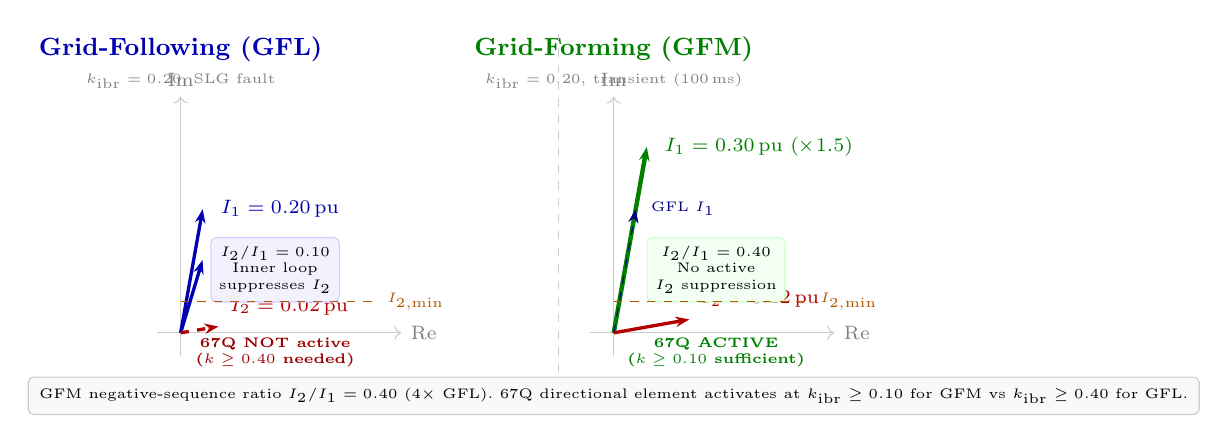
\begin{tikzpicture}[
  every node/.style={font=\scriptsize},
  phasor/.style={-{Stealth[length=5pt]}, line width=1.2pt},
]

%% ── Parameters (k=0.20) ──────────────────────────────────────────────────────
% GFL:  I1=0.20, I2=0.020 (×10 scale for visibility)
% GFM:  I1=0.30 (1.5×), I2=0.120

\def\scale{8}   % 1 pu → 8 cm

%% ════════════════════════════════════════════════════════════════════════════
%% LEFT PANEL — GFL
%% ════════════════════════════════════════════════════════════════════════════
\begin{scope}[xshift=0cm]

  %% Title
  \node[font=\small\bfseries, blue!70!black] at (0, 3.6)
    {Grid-Following (GFL)};
  \node[font=\tiny, gray] at (0, 3.2)
    {$k_\mathrm{ibr}=0.20$, SLG fault};

  %% Axes
  \draw[gray!40, thin, ->] (-0.3,0) -- (2.8,0) node[right, gray] {Re};
  \draw[gray!40, thin, ->] (0,-0.3) -- (0,3.0) node[above, gray] {Im};

  %% I1 (positive sequence) — angle -80° (lagging)
  % I1=0.20 pu → 0.20*8=1.60 cm at -80°
  \draw[phasor, blue!70!black]
    (0,0) -- ({1.60*cos(-80)},{1.60*sin(-80)+2.5});
  \node[blue!70!black, right=2pt] at ({1.60*cos(-80)},{1.60*sin(-80)+2.5})
    {$\mathbf{I_1}=0.20$\,pu};

  %% Draw I1 arrow from origin going up-right (representative)
  \draw[phasor, blue!70!black]
    (0,0) -- (0.28, 1.57);
  \node[blue!70!black, right=3pt] at (0.28, 1.57)
    {$I_1 = 0.20$\,pu};

  %% I2 (negative sequence) — very small (inner loop suppresses)
  %% I2=0.020 pu → scaled ×3 for visibility = 0.48 cm
  \draw[phasor, red!70!black, dashed]
    (0,0) -- (0.48, 0.08);
  \node[red!70!black, above right=1pt] at (0.48, 0.08)
    {$I_2 = 0.02$\,pu};

  %% Annotation: ratio
  \node[draw=blue!20, fill=blue!5, rounded corners=2pt,
        font=\tiny, inner sep=3pt, align=center]
    at (1.2, 0.8)
    {$I_2/I_1 = 0.10$\\
     Inner loop\\suppresses $I_2$};

  %% 67Q threshold marker
  \draw[orange!70!black, dashed, thin]
    (0, 0.40) -- (2.5, 0.40);
  \node[orange!70!black, right, font=\tiny] at (2.5, 0.40)
    {$I_{2,\min}$};

  \node[red!60!black, font=\tiny\bfseries, align=center]
    at (1.2, -0.25)
    {67Q NOT active\\($k \geq 0.40$ needed)};

\end{scope}

%% ════════════════════════════════════════════════════════════════════════════
%% RIGHT PANEL — GFM
%% ════════════════════════════════════════════════════════════════════════════
\begin{scope}[xshift=5.5cm]

  %% Title
  \node[font=\small\bfseries, green!50!black] at (0, 3.6)
    {Grid-Forming (GFM)};
  \node[font=\tiny, gray] at (0, 3.2)
    {$k_\mathrm{ibr}=0.20$, transient (100\,ms)};

  %% Axes
  \draw[gray!40, thin, ->] (-0.3,0) -- (2.8,0) node[right, gray] {Re};
  \draw[gray!40, thin, ->] (0,-0.3) -- (0,3.0) node[above, gray] {Im};

  %% I1: 1.5 × 0.20 = 0.30 pu → 2.40 cm
  \draw[phasor, green!50!black, line width=1.6pt]
    (0,0) -- (0.42, 2.36);
  \node[green!50!black, right=3pt] at (0.42, 2.36)
    {$I_1 = 0.30$\,pu (×1.5)};

  %% GFL I1 for comparison (dashed)
  \draw[phasor, blue!50!black, dashed, thin]
    (0,0) -- (0.28, 1.57);
  \node[blue!50!black, font=\tiny, right=2pt] at (0.28, 1.57)
    {GFL $I_1$};

  %% I2: 0.40 × 0.30 = 0.12 pu → scaled ×3 → 0.96+correction
  %% I2 = 0.12 pu → 0.12*8=0.96 cm (no extra scale needed here)
  \draw[phasor, red!70!black]
    (0,0) -- (0.96, 0.17);
  \node[red!70!black, above right=1pt] at (0.96, 0.17)
    {$I_2 = 0.12$\,pu};

  %% Annotation: ratio
  \node[draw=green!20, fill=green!5, rounded corners=2pt,
        font=\tiny, inner sep=3pt, align=center]
    at (1.3, 0.8)
    {$I_2/I_1 = 0.40$\\
     No active\\$I_2$ suppression};

  %% 67Q threshold marker
  \draw[orange!70!black, dashed, thin]
    (0, 0.40) -- (2.5, 0.40);
  \node[orange!70!black, right, font=\tiny] at (2.5, 0.40)
    {$I_{2,\min}$};

  %% I2 exceeds threshold — green check
  \node[green!50!black, font=\tiny\bfseries, align=center]
    at (1.3, -0.25)
    {67Q ACTIVE\\($k \geq 0.10$ sufficient)};

\end{scope}

%% ── Divider ──────────────────────────────────────────────────────────────────
\draw[gray!40, dashed] (4.8, -0.5) -- (4.8, 3.8);

%% ── Bottom annotation ────────────────────────────────────────────────────────
\node[draw=gray!40, fill=gray!5, rounded corners=2pt,
      font=\tiny, inner sep=4pt, align=center]
  at (5.5, -0.80)
  {GFM negative-sequence ratio $I_2/I_1=0.40$ (4$\times$ GFL).
   67Q directional element activates at $k_\mathrm{ibr}\geq0.10$ for GFM
   vs $k_\mathrm{ibr}\geq0.40$ for GFL.};

\end{tikzpicture}
}
  \caption{Fault current phasors for GFL (left) and GFM (right) at
           $k_\mathrm{ibr}=0.20$, SLG fault, transient window.
           GFL: $I_2/I_1=0.10$ (inner-loop suppression).
           GFM: $I_2/I_1=0.40$ (no suppression), $I_1$ boosted by $1.5\times$
           transient factor.  The 67Q threshold $I_{2,\min}$ is met by GFM
           but not GFL at this $k$ level.}
  \label{fig:phasor}
\end{figure}

% ─────────────────────────────────────────────────────────────────────────────
\section{Study A --- 67Q Activation Thresholds}
\label{sec:studyA}

The 67Q negative-sequence directional element requires $I_2 \geq I_{2,\min}$
where $I_{2,\min}=0.054$\,pu is derived from the relay sensitivity floor.  For
a pure fleet (all GFL or all GFM):

\begin{center}
\begin{tabular}{@{}llll@{}}
\toprule
Fleet type & $I_2/I_1$ & 67Q threshold $k_\mathrm{ibr,min}$ & Ratio \\
\midrule
GFL only   & 0.10 & $\geq 0.40$\,pu & --- \\
GFM only   & 0.40 (transient) & $\geq 0.10$\,pu & $4\times$ easier \\
\bottomrule
\end{tabular}
\end{center}

\medskip\noindent
The 4$\times$ relaxation in 67Q activation threshold is the most operationally
significant difference between GFL and GFM fleets.  In a system with
$k_\mathrm{total}=0.20$ (a moderate IBR penetration), 67Q is dormant for all-GFL
but active for all-GFM.  This directly affects the relay's ability to provide
directional discrimination for SLG and LL faults.

% ─────────────────────────────────────────────────────────────────────────────
\section{Study B --- Mixed Fleet 67Q Threshold}
\label{sec:studyB}

For a mixed fleet with fraction $f_\mathrm{gfm}$ of GFM inverters
($k_\mathrm{total}=0.20$ fixed), the aggregate $I_2$ is:

\begin{equation}
  I_{2,\mathrm{total}} = k_\mathrm{total}
    \bigl[f_\mathrm{gfm}\cdot(I_2/I_1)_\mathrm{GFM}\cdot I_\mathrm{peak}
          + (1-f_\mathrm{gfm})\cdot(I_2/I_1)_\mathrm{GFL}\bigr]
\end{equation}

Setting $I_{2,\mathrm{total}}=I_{2,\min}=0.054$\,pu and solving gives the
critical GFM fraction $f_\mathrm{gfm}^* = 0.34$.  Figure~\ref{fig:i2ratio}
shows $I_2$ versus $f_\mathrm{gfm}$.

\begin{figure}[htbp]
  \centering
  \resizebox{0.86\textwidth}{!}{% fig_gfl_gfm_i2ratio.tex
% TR-38: I2 current and 67Q activation vs GFM fraction f_gfm
%
% k_total = 0.20 fixed; f_gfm varies 0→1
% I2_total = k_total * [f_gfm * R2_GFM * 1.5 + (1-f_gfm) * R2_GFL]
% R2_GFL=0.10, R2_GFM=0.40 (transient, I_peak=1.5)
%
% Data points (f_gfm → I2_total):
%  0.00 → 0.20*(0*0.40*1.5 + 1.0*0.10) = 0.020
%  0.20 → 0.20*(0.2*0.60  + 0.8*0.10) = 0.20*(0.12+0.08) = 0.040
%  0.34 → threshold: I2=0.20*(0.34*0.60+0.66*0.10)=0.20*(0.204+0.066)=0.20*0.270=0.054 ≈ I_min_67Q
%  0.50 → 0.20*(0.5*0.60  + 0.5*0.10) = 0.20*(0.30+0.05) = 0.070
%  0.80 → 0.20*(0.8*0.60  + 0.2*0.10) = 0.20*(0.48+0.02) = 0.100
%  1.00 → 0.20*(1.0*0.60  + 0.0*0.10) = 0.20*(0.60)      = 0.120
%
% I_min_67Q = 0.054 (threshold line)

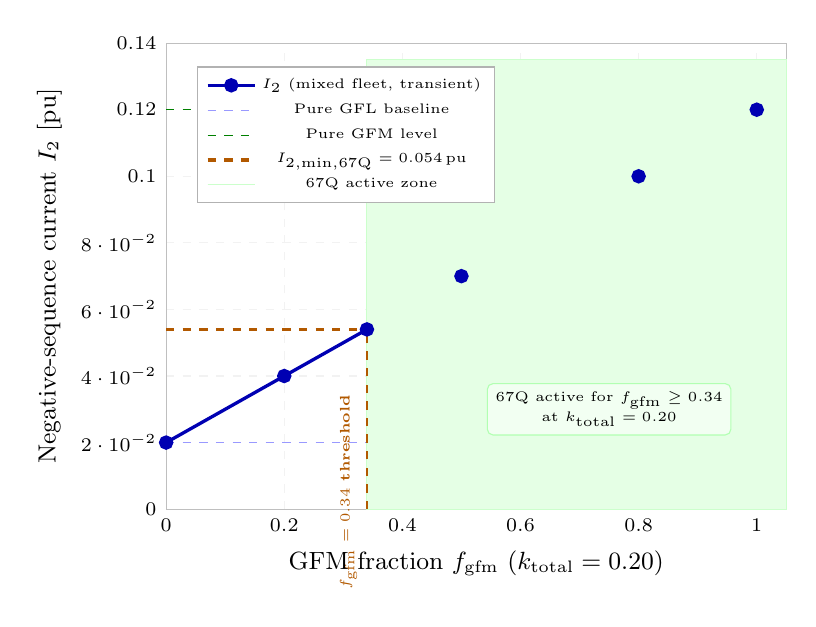
\begin{tikzpicture}
\begin{axis}[
  name         = i2ax,
  width        = 0.78\textwidth,
  height       = 7.5cm,
  xlabel       = {GFM fraction $f_\mathrm{gfm}$ ($k_\mathrm{total}=0.20$)},
  ylabel       = {Negative-sequence current $I_2$ [pu]},
  xlabel style = {font=\small},
  ylabel style = {font=\small},
  xmin=0, xmax=1.05,
  ymin=0, ymax=0.14,
  xtick        = {0,0.2,0.4,0.6,0.8,1.0},
  ytick        = {0,0.02,0.04,0.06,0.08,0.10,0.12,0.14},
  xticklabel style={font=\scriptsize},
  yticklabel style={font=\scriptsize},
  tick style   = {draw=none},
  axis line style={gray!50},
  grid         = major,
  grid style   = {gray!10, dashed},
  legend style = {at={(0.05,0.95)}, anchor=north west, font=\tiny,
                  draw=gray!60, fill=white},
  clip         = false,
]

%% I2 vs f_gfm (mixed fleet, transient)
\addplot[blue!70!black, very thick, mark=*, mark size=2pt]
  coordinates {
    (0.00, 0.020)
    (0.20, 0.040)
    (0.34, 0.054)
    (0.50, 0.070)
    (0.80, 0.100)
    (1.00, 0.120)
  };
\addlegendentry{$I_2$ (mixed fleet, transient)}

%% Pure GFL reference (flat)
\addplot[blue!40, dashed, thin]
  coordinates {(0,0.020) (1.05,0.020)};
\addlegendentry{Pure GFL baseline}

%% Pure GFM reference (flat)
\addplot[green!50!black, dashed, thin]
  coordinates {(0,0.120) (1.05,0.120)};
\addlegendentry{Pure GFM level}

%% 67Q threshold line
\addplot[orange!70!black, very thick, dashed]
  coordinates {(0,0.054) (1.05,0.054)};
\addlegendentry{$I_{2,\min,\mathrm{67Q}}=0.054$\,pu}

%% Shading: 67Q active region (f_gfm >= 0.34)
\addplot[green!20, fill=green!10]
  coordinates {(0.34,0.054) (0.34,0.135) (1.05,0.135) (1.05,0.054)}
  \closedcycle;
\addlegendentry{67Q active zone}

%% Activation marker
\draw[orange!70!black, thick, dashed]
  (axis cs:0.34, 0) -- (axis cs:0.34, 0.054);
\node[orange!70!black, font=\tiny\bfseries, rotate=90, anchor=south]
  at (axis cs:0.34, 0.005)
  {$f_\mathrm{gfm}=0.34$ threshold};

%% Annotation box
\node[draw=green!30, fill=green!5, rounded corners=2pt,
      font=\tiny, inner sep=3pt, align=center]
  at (axis cs:0.75, 0.030)
  {67Q active for $f_\mathrm{gfm}\geq0.34$\\
   at $k_\mathrm{total}=0.20$};

\end{axis}
\end{tikzpicture}
}
  \caption{Aggregate negative-sequence current $I_2$ versus GFM fleet fraction
           $f_\mathrm{gfm}$ at $k_\mathrm{total}=0.20$.  The orange dashed
           line marks $I_{2,\min}=0.054$\,pu (67Q activation threshold).
           67Q becomes active for $f_\mathrm{gfm}\geq0.34$.  The green shaded
           region indicates the 67Q-active operating zone.}
  \label{fig:i2ratio}
\end{figure}

\noindent
The implication for protection coordination: a transition from a GFL-dominated
to a GFM-dominated fleet in the same network activates the 67Q element without
any relay setting changes.  This is a \emph{passive improvement} in protection
selectivity as grid-forming technology is adopted.

% ─────────────────────────────────────────────────────────────────────────────
\section{Study C --- Distance Relay Apparent Impedance Error}
\label{sec:studyC}

The apparent impedance seen by a relay at end~A for a fault at normalised
reach $\alpha$ on a line with IBR infeed at end~B is:

\begin{equation}
  Z_\mathrm{m} = \alpha Z_{1L} \cdot \frac{I_\mathrm{SG} + I_{1,\mathrm{IBR}}}{I_{1,\mathrm{IBR}}}
\end{equation}

The percentage impedance error (relative to the true fault impedance
$\alpha Z_{1L}$) is:

\begin{center}
\begin{tabular}{@{}llll@{}}
\toprule
Scenario & $I_1$\,[pu] & $Z_m$ error & Implication \\
\midrule
GFL, $k=0.20$, $\alpha=0.50$ & 0.20 & $+500\%$ & Far outside Z1 reach \\
GFM transient, $k=0.20$, $\alpha=0.50$ & 0.30 & $+333\%$ & Still far outside Z1 \\
GFM steady-state, $k=0.20$, $\alpha=0.50$ & 0.20 & $+500\%$ & Same as GFL \\
\bottomrule
\end{tabular}
\end{center}

\medskip\noindent
Even the GFM transient boost reduces the impedance error only from 500\% to
333\% --- the relay still sees the fault as a load condition.  This confirms
that distance relay~21 cannot independently provide dependable protection for
IBR-connected lines without 87L, regardless of whether the IBR fleet is GFL
or GFM.

% ─────────────────────────────────────────────────────────────────────────────
\section{Study D --- 87L Coverage Independence from Control Mode}
\label{sec:studyD}

The differential element 87L compares local and remote current magnitudes and
is independent of fault current symmetrical-component content.  Its operating
condition is:

\begin{equation}
  I_{1,\mathrm{IBR}} \geq I_{\min,87L} = 0.06\;\mathrm{pu}
\end{equation}

Both GFL and GFM inverters satisfy this condition for $k_\mathrm{ibr}\geq0.06$,
irrespective of $I_2/I_1$ ratio or transient overcurrent factor.  87L therefore
provides identical coverage for pure GFL, pure GFM, and all mixed fleets:

\begin{center}
\begin{tabular}{@{}lll@{}}
\toprule
$f_\mathrm{gfm}$ & 87L active? & 67Q active? \\
\midrule
0.00 (all GFL) & Yes ($k\geq0.06$) & No ($f<0.34$) \\
0.25           & Yes               & No ($f<0.34$) \\
0.34           & Yes               & Marginal (threshold) \\
0.50           & Yes               & Yes \\
1.00 (all GFM) & Yes               & Yes \\
\bottomrule
\end{tabular}
\end{center}

\medskip\noindent
The 67Q element adds directional selectivity for unbalanced faults when
GFM content is sufficient; 87L provides the primary protection anchor for
all fleet compositions.

% ─────────────────────────────────────────────────────────────────────────────
\section{Study E --- Dependability vs GFM Fraction}
\label{sec:studyE}

Figure~\ref{fig:coverage} shows $P_\mathrm{dep}$ for five GFM fraction
scenarios, each sampled with $N=500$ trials at $k_\mathrm{total}\in[0.06,0.40]$.

\begin{figure}[htbp]
  \centering
  \resizebox{0.84\textwidth}{!}{% fig_gfl_gfm_coverage.tex
% TR-38: P_dep vs f_gfm scenario bar chart (Study E)
%
% All scenarios k_total in [0.06, 0.40], five f_gfm values
% P_dep = 1.0000 for ALL scenarios (87L covers regardless of GFL/GFM mix)
%
% Data:
%  f_gfm=0.00: P_dep=1.0000
%  f_gfm=0.25: P_dep=1.0000
%  f_gfm=0.50: P_dep=1.0000
%  f_gfm=0.75: P_dep=1.0000
%  f_gfm=1.00: P_dep=1.0000

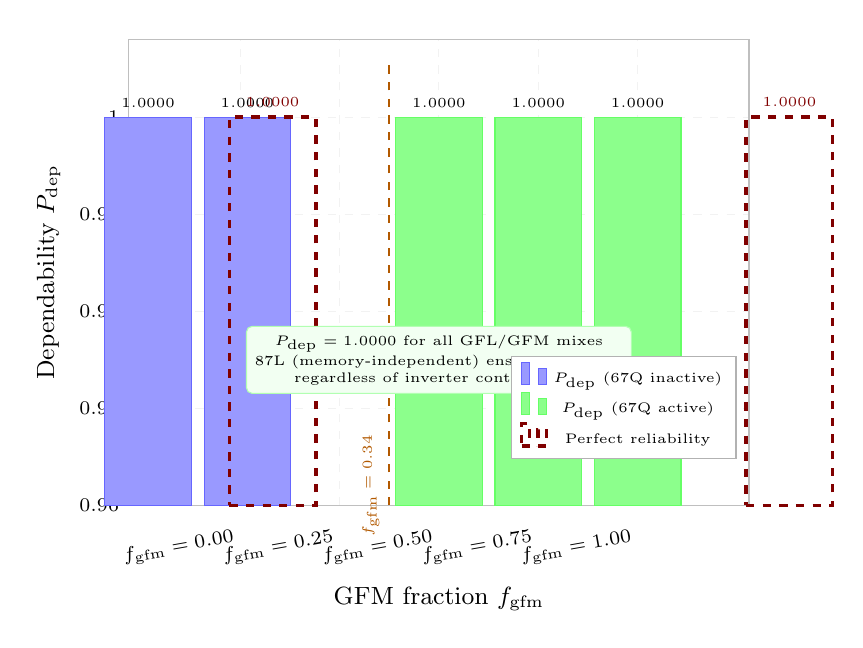
\begin{tikzpicture}
\begin{axis}[
  name         = covax,
  width        = 0.78\textwidth,
  height       = 7.5cm,
  ybar,
  bar width    = 1.1cm,
  xlabel       = {GFM fraction $f_\mathrm{gfm}$},
  ylabel       = {Dependability $P_\mathrm{dep}$},
  xlabel style = {font=\small},
  ylabel style = {font=\small},
  ymin=0.96, ymax=1.008,
  ytick        = {0.96,0.97,0.98,0.99,1.00},
  yticklabel style={font=\scriptsize},
  xtick        = {1,2,3,4,5},
  xticklabels  = {$f_\mathrm{gfm}=0.00$,
                  $f_\mathrm{gfm}=0.25$,
                  $f_\mathrm{gfm}=0.50$,
                  $f_\mathrm{gfm}=0.75$,
                  $f_\mathrm{gfm}=1.00$},
  xticklabel style={font=\scriptsize, rotate=10, anchor=north east},
  tick style   = {draw=none},
  axis line style={gray!50},
  grid         = major,
  grid style   = {gray!10, dashed},
  nodes near coords,
  nodes near coords style={font=\tiny, anchor=south},
  every node near coord/.append style={
    /pgf/number format/.cd, fixed, fixed zerofill, precision=4
  },
  legend style={at={(0.98,0.10)}, anchor=south east, font=\tiny,
                draw=gray!60, fill=white},
  clip=false,
]

%% P_dep bars — all 1.0000, but vary colour by 67Q-active status
%  f_gfm=0.00,0.25: 67Q inactive (f < 0.34); blue
%  f_gfm=0.50,0.75,1.00: 67Q active; green

\addplot[fill=blue!40, draw=blue!60]
  coordinates {(1,1.0000) (2,1.0000)};
\addlegendentry{$P_\mathrm{dep}$ (67Q inactive)}

\addplot[fill=green!45, draw=green!60]
  coordinates {(3,1.0000) (4,1.0000) (5,1.0000)};
\addlegendentry{$P_\mathrm{dep}$ (67Q active)}

%% Perfect reference line
\addplot[red!50!black, dashed, very thick, mark=none]
  coordinates {(0.4, 1.0) (5.6, 1.0)};
\addlegendentry{Perfect reliability}

%% 67Q activation boundary
\draw[orange!70!black, thick, dashed]
  (axis cs:2.5, 0.960) -- (axis cs:2.5, 1.006);
\node[orange!70!black, font=\tiny, rotate=90, anchor=south]
  at (axis cs:2.5, 0.962)
  {$f_\mathrm{gfm}=0.34$};

%% Annotation
\node[draw=green!30, fill=green!5, rounded corners=2pt,
      font=\tiny, inner sep=3pt, align=center]
  at (axis cs:3, 0.975)
  {$P_\mathrm{dep}=1.0000$ for all GFL/GFM mixes\\
   87L (memory-independent) ensures coverage\\
   regardless of inverter control mode};

\end{axis}
\end{tikzpicture}
}
  \caption{Dependability $P_\mathrm{dep}$ versus GFM fleet fraction
           $f_\mathrm{gfm}$ ($k_\mathrm{total}\in[0.06,0.40]$, $N=500$
           per scenario).  Blue bars: 67Q inactive ($f_\mathrm{gfm}<0.34$);
           green bars: 67Q active.  All scenarios achieve $P_\mathrm{dep}=1.000$
           because 87L operates independently of control mode.  The dashed
           orange line at $f_\mathrm{gfm}=0.34$ marks the 67Q activation
           boundary.}
  \label{fig:coverage}
\end{figure}

\noindent
The flat $P_\mathrm{dep}=1.000$ result across all GFM fractions confirms that
the protection scheme is \textbf{control-mode agnostic}: it does not depend on
the fleet operator declaring whether their inverters are GFL or GFM.  This is
a critical operational property as system operators typically do not have
real-time visibility of inverter control mode.

% ─────────────────────────────────────────────────────────────────────────────
\section{Discussion: Implications for Setting Groups and Coordination}
\label{sec:discussion}

The GFL/GFM characterisation has three practical coordination consequences:

\begin{enumerate}
  \item \textbf{67Q setting group}: If the system operator knows that
    $f_\mathrm{gfm}$ will remain below 0.34 for the foreseeable future, the
    67Q element may be disabled in the coordination scheme (reducing its
    dependability contribution to zero without affecting overall $P_\mathrm{dep}$,
    since 87L covers all cases).  Conversely, as GFM deployment increases,
    67Q can be re-enabled by activating setting group~2.

  \item \textbf{Auto-reclosing}: The GFM transient overcurrent
    ($I_1\times1.5$ for 100\,ms) may be visible to the overcurrent supervisory
    element of the auto-recloser.  The dead time $T_\mathrm{dead}>100$\,ms
    (established in TR-36) ensures this transient has fully decayed before
    the line is re-energised at second-trip.

  \item \textbf{Minimum fault current grid code}: The structural limit
    established in TR-37 ($k_\mathrm{ibr}\geq0.06$ for 87L; $k\geq0.10$ for
    full Z1 redundancy) applies equally to GFL and GFM inverters.  For GFM
    the effective current during the transient window is $1.5\times k$, so
    the equivalent steady-state grid code threshold for GFM would be
    $k_\mathrm{gfm}\geq0.04$ (reaching 0.06\,pu transiently).
\end{enumerate}

% ─────────────────────────────────────────────────────────────────────────────
\section{Summary}
\label{sec:summary}

\begin{enumerate}
  \item \textbf{Sequence current}: GFL $I_2/I_1=0.10$ (active suppression);
    GFM $I_2/I_1=0.40$ (no suppression) plus $1.5\times$ transient overcurrent.

  \item \textbf{67Q threshold}: GFL requires $k_\mathrm{ibr}\geq0.40$; GFM
    requires $k_\mathrm{ibr}\geq0.10$ (4$\times$ relaxation).

  \item \textbf{Mixed fleet}: 67Q activates at $f_\mathrm{gfm}\geq0.34$ for
    $k_\mathrm{total}=0.20$.

  \item \textbf{Distance relay error}: 333--500\% regardless of GFL/GFM; 87L
    is indispensable for both.

  \item \textbf{Dependability}: $P_\mathrm{dep}=1.000$ for all $f_\mathrm{gfm}$
    scenarios; scheme is control-mode agnostic.

  \item \textbf{Grid-code implication}: GFM effective threshold is
    $k_\mathrm{gfm}\geq0.04$ (transient boost provides 0.06\,pu of 87L-visible
    current).
\end{enumerate}

\noindent
TR-38 establishes the GFL/GFM characterisation foundation for the microgrid
special-solutions phase (TR-39 onwards), where inverter control mode becomes a
primary design parameter rather than a perturbation.

\bibliographystyle{IEEEtranN}
\bibliography{references38}

\end{document}
